% Nama Kelompok : Kelompok 3
% Kelas : D4 TI 1A
% 1. Kadek Diva Krishna Murti (1174006)
% 2. Niko
% 3. Rizal Rony Sitorus
% 4. Jeremia
% 5. Sri Rahayu (1174015)

\begin{figure}[ht]
\centerline{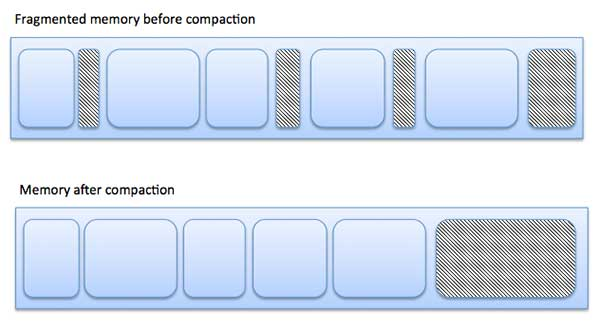
\includegraphics[width=1\textwidth]{figures/fragmentation.jpg}}
\caption{Contoh fragmentasi.}
\label{fragmentasi}
\end{figure}

\section{Definisi Fragmentasi}
Fragmentasi \ref{fragmentasi} merupakan suatu kejadian pada ruang penyimpanan di mana ruang penyimpanan dipergunakan secara tidak efisien dan mengurangi kapasitas penyimpanan. Istilah fragmentasi ini dipergunakan untuk merujuk pada tempat yang gersang itu sendiri. Dapat disimpulkan bahwa fragmentasi adalah munculnya lubang-lubang yang tidak cukup besar untuk menampung permintaan dari proses.

\section{Jenis-Jenis Fragmentasi}
Fragmentasi dapat berupa fragmentasi internal maupun fragmentasi eksternal.
\subsection{Fragmentasi Internal}
Berdasarkan buku yang berjudul Sistem Operasi \cite{pangera2005sistem} fragmentasi internal adalah tidak efisiennya utilitas memori utama di mana sembarang program sekecil apapun tidak bergantung, akan menempati seluruh partisi. Keadaan ini mengakibatkan pemborosan ruang yang bersifat internal terhadap partisi dengan kenyataan di mana blok data yang dimuatkan berukuran lebih kecil dari partisi.

Fragmentasi internal terjadi ketika jumlah memori yang ditentukan oleh CPU untuk nantinya ditempati oleh proses lebih besar dari pada yang diminta oleh proses itu sendiri dikarenakan adanya selisih diantara permintaan proses dengan alokasi lubang yang sudah ditetapkan, namun untuk satu partisi tertentu hanya berukuran kecil sehingga tidak dipergunakan. Hal ini umumnya terjadi ketika kita menggunakan sistem partisi banyak tetap. Contoh dari kejadian tersebut, yaitu ketika di mana ada proses dengan permintaan memori sebesar 18 KB, lalu memori akan dipartisi menjadi blok - blok yang masing-masing besarnya 5 KB. Pada sistem partisi banyak tetap, memori yang dialokasikan untuk proses adalah 4 blok, atau sebesar 20 KB. Padahal, yang nantinya terpakai hanya sebesar 18 KB dan sisanya sebesar 2 KB tetap diberikan pada proses tersebut, walaupun tidak akan terpakai oleh proses tersebut. Hal ini berarti pula proses lain tidak dapat memakainya. Perbedaan memori yang dialokasikan dengan yang diminta inilah yang disebut fragmentasi internal.p Sebagai contoh, pada multiple partition fragmentasi internal mungkin terjadi pada situasi berikut. Terdapat lubang sebanyak 18463 byte dan proses meminta sebanyak 18461 byte seperti yang terjadi pada Gambar \ref{fragmentasiinternal}. Maka alokasi yang dilakukan disesuaikan dengan permintaan dan nantinya akan tersisa lubang sebanyak 2 byte. Penyimpanan lubang ini akan memerlukan memori lebih besar dari lubang itu sendiri. Pendekatannya adalah dengan mengalokasikan lubang yang sangat kecil sebagai bagian dari permintaan yang besar.

Fragmentasi internal tidak dapat dihindarkan apabila kita menggunakan sistem partisi banyak berukuran tetap, mengingat besar lubang - lubang yang disediakan selalu tetap, kecuali jika kita menggunakan sistem partisi banyak dinamis, yang memungkinkan suatu proses untuk diberikan ruang memori sebesar yang dia minta.

\subsection{Fragmentasi Eksternal}
Berdasarkan buku yang berjudul Sistem Operasi \cite{pangera2005sistem} fragmentasi eksternal adalah keadaan di mana suatu proses pada awalnya berjalan dan bekerja dengan baik, namun ketika mengarah ke situasi yang di mana terdapat banyak lubang - lubang kecil di dalam sebuah memori sehingga semakin lama memori tersebut semakin terfragmentasi dan utilisasi memori pun kinerjanya menjadi menurun sehubungan dengan kenyataan bahwa memori bersifat eksternal terhadap semua partisi menjadi sangat terfragmentasi. Keadaan ini merupakan kebalikan dari fragmentasi ini.

Fragmentasi eksternal terjadi pada saat di mana jumlah keseluruhan memori kosong yang tersedia memang mencukupi untuk menampung permintaan tempat dari proses, tetapi tidak dapat dialokasikan karena letaknya tidak berkesinambungan atau tidak berurutan atau terpecah menjadi beberapa bagian kecil sehingga proses tidak dapat masuk. Umumnya, ini terjadi ketika kita menggunakan sistem partisi banyak dinamis. Seperti yang diperumpamakan sebelumnya, pada sistem partisi banyak dinamis sistem akan terbagi menjadi blok - blok yang besarnya tidak tetap. Maksud dari tidak tetapi adalah blok tersebut bisa bertambah menjadi besar atau bertambah menjadi kecil. 

Sebagai perumpamaan, sebuah proses meminta ruang memori sebanyak 18 KB, sedangkan memori nantinya akan dipartisi menjadi blok - blok yang besarnya masing - masing sebanyak 5 KB, maka yang nantinya akan diberikan proses adalah 3 blok ditambah 2 KB dari sebuah blok. Lalu sisa blok yang banyaknya 2 KB akan dipersiapkan guna menampung proses lainnya atau jika nantinya bertentangga dengan ruang memori yang kosong, maka akan bergabung dengan ruang memori yang kosong tersebut. Akibatnya dengan sistem partisi banyak dinamis, bisa tercipta lubang-lubang di memori, yaitu ruang memori yang kosong. Keadaan saat lubang-lubang ini tersebar yang masing-masing lubang tersebut tidak ada yang bisa memenuhi kebutuhan proses padahal jumlah dari besarnya lubang tersebut cukup untuk memenuhi kebutuhan proses disebut sebagai fragmentasi eksternal. Fragmentasi eksternal dilakukan pada algoritma alokasi dinamis, terutama strategi first-fit dan best-fit.

Fragmentasi eksternal dapat diatasi dengan beberapa cara, diantaranya adalah :

\begin{enumerate}

\item Compaction atau Pemadatan\\
Compaction atau Pemadatan, yaitu memadatkan atau mengatur kembali isi memori agar memori yang kosong diletakkan bersama di suatu bagian yang besar sehingga proses dapat masuk ke ruang memori kosong tersebut. Proses pemadatan dapat dilakukan apabila relokasinya bersifat dinamis dan pengalamatan programnya dilakukan pada saat program tersebut dieksekusi. Kebutuhan akan pemadatan akan hilang bila pengalamatan dapat dilakukan secara berurutan, walaupun sebenarnya proses tidak ditempatkan pada lokasi memori yang berurutan. Nantinya, konsep ini diterapkan dengan Paging. Pemadatan tidak selalu dapat dipakai. Supaya proses nantinya dapat dieksekusi pada lokasi baru, maka semua alamat internal harus direlokasi. Proses pemadatan hanya dapat dilakukan pada relokasi dinamis saja dan dikerjakan pada saat program dieksekusi dikarenakan untuk melakukan relokasi dibutuhkan pemindahan program dan data, lalu kemudian mengubah register basis (relokasi) yang mencerminkan alamat basis baru. Terdapat beberapa cara pemadatan seperti pada Gambar \ref{pemadatan}.

\begin{figure}[ht]
\centerline{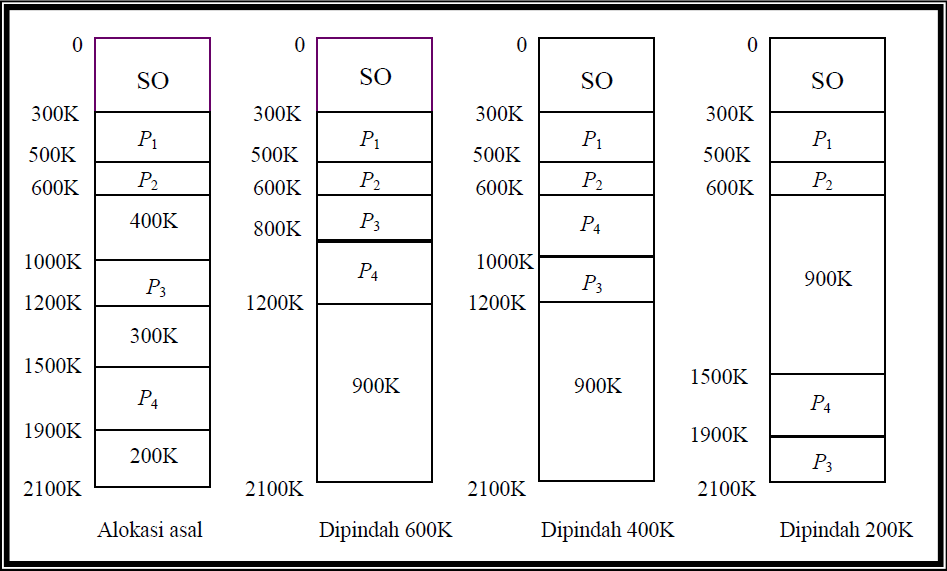
\includegraphics[width=1\textwidth]{figures/pemadatan.png}}
\caption{Compaction atau Pemadatan.}
\label{pemadatan}
\end{figure}


\item Penghalaman atau Paging \\
Penghalaman atau paging  merupakan metode yang memungkinkan suatu alamat fisik memori yang tersedia dapat tidak berurutan. Pemberian halaman bisa menjadi jalan keluar untuk memcahkan masalah luar. Untuk bisa mengimplementasikan solusi ini bisa melalui pengunaan dari skema pemberian halaman. Dengan pemberian halaman ini nantinya dapat mencegah masalah - masalah penting dari pemuatan besar ukuran memori yang bervariasi kedalam penyimpanan cadangan. Ketika beberapa pecahan kode dari data yang tersisa di memori utama diperlukan untuk ditukar keluar, maka harus ditemukan ruang yang akan dipergunakan sebagai penyimpanan cadangan tersebut nantinya. Bagian yang nantinya dipergunakan guna menunjang pemberian halaman telah ditangani oleh perangkat keras. Konsep yang ada baru - baru ini telah diimplementasikan dengan menggabungkan perangkat keras dan sistem operasi, terutama pada microprocessor 64 bit.

%%%%%%%%%%%%%%%%%%%%%%%%%%%%%%%

\item Segmentasi\\
Segmentasi adalah sebuah skema manajemen memori yang mendukung cara pandang seorang programmer terhadap memori. Ruang alamat logika merupakan sekumpulan dari segmen-segmen. Masing-masing segment mempunyai panjang dan nama. Alamat diartikan sebagai nama segmen dan offset dalam suatu segmen. Jika seorang user ingin menunjuk sebuah alamat, maka dapat dilakukan dengan cara menunjuk nama segment dan offsetnya. Untuk lebih menyederhanakan implementasi, segment - segment nantinya diberi nomor yang di mana nomor tersebut dipergunakan sebagai pengganti nama segment. Sehingga nantinya alamat logika terdiri dari dua tupple: [segment-number, offset].
\end{enumerate}

\begin{figure}[ht]
\centerline{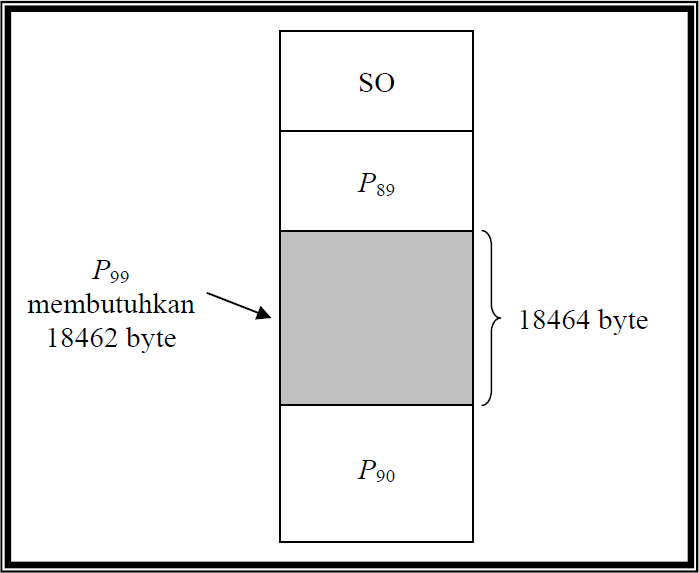
\includegraphics[width=1\textwidth]{figures/fragmentasi_internal.png}}
\caption{Fragmentasi Internal.}
\label{fragmentasiinternal}
\end{figure}

\subsection{Fragmentasi Data}

Data fragmentasi terjadi ketika sebuah bagian dari data dalam memori rusak ke dalam banyak potongan-potongan yang tidak saling berdekatan. Kejadian tersebut terjadi dari hasil mencoba untuk memasukkan benda yang besar ke dalam penyimpanan yang telah terjadi fragmentasi eksternal sebelumnya.

Misalnya, file dalam file sistem biasanya diatur dalam unit yang disebut blok atau kelompok. Ketika sebuah file sistem dibuat, ada ruang untuk menyimpan file blok bersama contiguously. Hal tersebut memungkinkan terjadinya proses membaca dan menulis file cepat berurut. Namun, seperti file ditambahkan, dihapus, dan berubah dalam ukuran, ruang bagi menjadi eksternal, hanya meninggalkan lubang kecil di tempat yang tepat untuk data baru. Jika file yang baru dibuat, lalu ditulis atau jika file yang sudah ada ditambahkan, maka data baru blok akan tersebar dikarenakan lambatnya akses untuk mencari waktu dan pemutaran penundaan dari membaca atau menulis head dan overhead incurring tambahan untuk mengelola tambahan lokasi. Hal ini disebut fragmentasi file system.

Contoh lainnya, bila sebuah node yang terhubung turut didaftarkan dan dialokasikan dalam memori, hal tersebut akan meningkatkan lokalitas dari referensi dan meningkatkan kinerja data cache selama traversal dari daftar. Jika memori memang gratis bagi ruang, maka node akan tersebar di seluruh memori dan meningkatkan jumlah cache misses.

Seperti pemadatan yang dapat menghilangkan fragmentasi eksternal, data fragmentasi juga dapat dihapuskan oleh rearranging data terkait agar saling berdekatan. Misalnya, pekerjaan utama dari defragmentation adalah untuk mengatur ulang blok pada disk, sehingga setiap file blok saling berdekatan. Defragmenting juga berusaha mengurangi atau menghilangkan fragmentasi ruang kosong. Beberapa objek dipindahkan agar lebih dekat (Pemadatan) untuk meningkatkan kinerja cache.

\section{Kesimpulan}

Algoritma alokasi penyimpanan dinamis mana pun yang digunakan, tetap tidak bisa menutup kemungkinan terjadinya fragmentasi. Bahkan hal ini bisa menjadi fatal. Salah satu kondisi terburuk adalah apabila kita memiliki memori terbuang setiap dua proses. Apabila semua memori - memori yang terbuang itu digabungkan, maka bukan tidak mungkin akan cukup untuk menampung sebuah proses. Sebuah contoh statistik menunjukkan bahwa saat menggunakan metoda first fit, bahkan setelah dioptimisasi, dari N blok teralokasi, sebanyak 0.5N blok lain akan terbuang karena fragmentasi. Jumlah sebanyak itu berarti kurang lebih setengah dari memori tidak dapat digunakan. Hal ini disebut dengan aturan 50\%.
\\
\\
Beberapa jenis strategi pencocokan antara lain:
\begin{table}[h!]
\centering
\begin{tabular}{ |c|c|l| }
\hline
1 & Cocok pertama (first fit) & Pencocokan terjadi menurut antrian informasi \\
\hline
2 & Cocok pertama berdaur (cyclical first fit) &  Pencocokan tidak harus dimulai dari urutan penggalan memori yang pertama, tetapi dapat dilakukan setelah terjadi pencocokan sebelumnya. \\
\hline
3 & Cocok terbaik (best fit) &  Pencocokan dilakukan sesuai dengan penggalan memori yang ukurannya pas. \\
\hline
4 & Cocok terburuk (Worst fit) & Informasi akan menempati penggalan yang ukurannya terbesar. \\
\hline
\end{tabular}
\end{table}
